%%
%% EmPath: Multimodal Pain Intensity Detection Using Biosignals and Facial Landmarks
%% ACM SAC 2027 — Bioinformatics, Computational Biology, and Biomedical Informatics (BCB) Track
%%
%% Authors: Komala Belur Srinivas, Purna Prasad
%%          Department of Computer Science, Hofstra University
%%
%% SUBMISSION NOTE:
%%   - For double-blind review, change to: \documentclass[sigconf,anonymous]{acmart}
%%   - Remove the 'review' option for camera-ready
%%   - Verify CCS concepts at https://dl.acm.org/ccs
%%   - Page limit: 8 pages + references (SAC BCB track)
%%

\documentclass[sigconf]{acmart}

%% ---- Packages ---------------------------------------------------------------
\usepackage{booktabs}       % professional tables
\usepackage{microtype}      % better typography
\usepackage{balance}        % balance last-page columns
\usepackage{multirow}       % table multirow
\usepackage{graphicx}       % figures
\usepackage{xspace}         % smart spacing
\usepackage{url}            % \url{} for code links

%% ---- ACM Metadata -----------------------------------------------------------
\acmConference[SAC '27]{The 42nd ACM/SIGAPP Symposium on Applied Computing}
              {March 2027}{Bonn, Germany}
\acmYear{2027}
\copyrightyear{2027}
%% Leave DOI/ISBN blank — ACM fills these in after acceptance
\acmISBN{978-x-xxxx-xxxx-x/27/03}
\acmDOI{10.1145/xxxxxxx.xxxxxxx}

%% ---- CCS Concepts -----------------------------------------------------------
%% Generated at https://dl.acm.org/ccs
\begin{CCSXML}
<ccs2012>
  <concept>
    <concept_id>10010147.10010257.10010293.10010294</concept_id>
    <concept_desc>Computing methodologies~Ensemble methods</concept_desc>
    <concept_significance>500</concept_significance>
  </concept>
  <concept>
    <concept_id>10010583.10010600.10010601</concept_id>
    <concept_desc>Applied computing~Health informatics</concept_desc>
    <concept_significance>500</concept_significance>
  </concept>
  <concept>
    <concept_id>10010147.10010257.10010321.10010331</concept_id>
    <concept_desc>Computing methodologies~Feature selection</concept_desc>
    <concept_significance>300</concept_significance>
  </concept>
  <concept>
    <concept_id>10010147.10010257.10010293.10010296</concept_id>
    <concept_desc>Computing methodologies~Random forests</concept_desc>
    <concept_significance>300</concept_significance>
  </concept>
</ccs2012>
\end{CCSXML}

\ccsdesc[500]{Computing methodologies~Ensemble methods}
\ccsdesc[500]{Applied computing~Health informatics}
\ccsdesc[300]{Computing methodologies~Feature selection}
\ccsdesc[300]{Computing methodologies~Random forests}

\keywords{pain detection; multimodal fusion; biosignals; facial landmarks;
          stacked generalization; leave-one-subject-out; SHAP; BioVid}

%% ---- Authors ----------------------------------------------------------------
\author{Komala Belur Srinivas}
\authornote{This work was conducted as a capstone research project.}
\email{kbelursrinivas1@pride.hofstra.edu}
\orcid{0000-0000-0000-0000}   %% replace with real ORCID if available
\affiliation{%
  \institution{Hofstra University}
  \department{Department of Computer Science}
  \city{Hempstead}
  \state{New York}
  \country{USA}
}

\author{Purna Prasad}
\authornotemark[1]
\email{purna.prasad@hofstra.edu}
\affiliation{%
  \institution{Hofstra University}
  \department{Department of Computer Science}
  \city{Hempstead}
  \state{New York}
  \country{USA}
}

%% ============================================================
\begin{document}
%% ============================================================

\title{EmPath: Multimodal Pain Intensity Detection Using\\
       Biosignals and Facial Landmarks}

%% ---- Abstract ---------------------------------------------------------------
\begin{abstract}
This paper presents EmPath, a multimodal machine learning system for
discriminating between adjacent pain intensity levels (PA2 and PA3) using the
BioVid Heat Pain Database. Physiological signals (galvanic skin response,
electrocardiogram, electromyography) and facial landmark trajectories extracted
via MediaPipe FaceMesh are processed into 35 biosignal and 22 landmark features
across 2,680 trials from 67 thermally reactive participants. A stacked
generalization framework combining two base Random Forest classifiers with a
Logistic Regression meta-learner is evaluated under strict
Leave-One-Subject-Out (LOSO) cross-validation. EmPath achieves 65.3\% mean
accuracy ($SD = 14.1\%$, $\text{AUC} = 0.719$, $F_1 = 0.653$), outperforming
biosignal-only ($63.1\% \pm 11.6\%$) and landmark-only ($61.4\% \pm 13.1\%$)
baselines. To our knowledge, this is the first reported LOSO result on the 67
thermally reactive subjects of BioVid for the PA2/PA3 boundary, establishing a
reproducible baseline for adjacent-level pain discrimination. SHAP analysis
identifies \texttt{gsr\_slope} as the dominant biosignal predictor and
\texttt{mouth\_height\_std} as the dominant facial landmark predictor. A
comprehensive ablation study across 26 architectural variants confirms the
stacked fusion configuration as optimal, with deep learning and foundation
model approaches consistently underperforming due to data sparsity under LOSO.
Code and pre-computed features are available at
\url{https://github.com/komala-b-srinivas/empath-pain-detection}.
\end{abstract}

\maketitle

%% ============================================================
\section{Introduction}
\label{sec:intro}
%% ============================================================

Pain is the most common reason patients seek medical care, yet its assessment
remains predominantly subjective, relying on self-report instruments such as
visual analog scales~\cite{jensen2003}. This creates a critical clinical gap
for patients who cannot self-report---including ICU-sedated individuals, those
with advanced dementia, neonates, and patients with severe communication
disorders~\cite{puntillo2004,lichtner2014}---who may receive inadequate
analgesia due to the absence of objective quantification tools.

The autonomic nervous system responds to nociceptive stimulation through
measurable changes in galvanic skin response (GSR), heart rate variability
(HRV), and electromyographic activity (EMG)~\cite{loggia2011}. Simultaneously,
pain produces characteristic facial muscle activations that are largely
involuntary and cross-culturally consistent~\cite{ekman1978,prkachin2008}.
These two signal streams carry complementary information: biosignals capture
systemic autonomic activation, while facial movements encode the expressive
component of the pain experience. Combining them through multimodal fusion
should, in principle, yield more reliable pain estimates than either channel
alone~\cite{werner2017}.

The BioVid Heat Pain Database~\cite{walter2013} provides a standardized
benchmark with synchronized physiological and video recordings from 87
participants. Discriminating between adjacent intensity levels PA2
($\approx 43^\circ$C) and PA3 ($\approx 44^\circ$C), which differ by
approximately 1$^\circ$C, represents a particularly challenging subproblem.
We address four contributions: (1)~a stacked generalization framework combining
modality-specific Random Forests; (2)~strict LOSO evaluation on 67 reactive
subjects; (3)~a comprehensive 26-variant ablation study spanning deep learning,
foundation models, and advanced fusion strategies; and (4)~SHAP-based feature
attribution providing physiologically interpretable insight.

%% ============================================================
\section{Related Work}
\label{sec:related}
%% ============================================================

\textbf{Biosignal-based pain detection.}
Kächele et al.~\cite{kachele2016} demonstrated that cross-subject
generalization on BioVid is substantially lower than within-subject
performance, confirming the difficulty of subject-independent evaluation.
Tavakolian et al.~\cite{tavakolian2020} achieved approximately 60\%
LOSO accuracy using frequency-domain HRV features combined with skin
conductance features. Foundation models pretrained on large biosignal
corpora (BIOT~\cite{yang2023}, PainFormer) underperform simple RF baselines
on BioVid~\cite{gkikas2023}, suggesting distribution mismatch with
heat-pain-elicited signals.

\textbf{Facial landmark-based pain recognition.}
The Facial Action Coding System (FACS)~\cite{ekman1978} characterizes pain
expression through Action Units including AU4 (brow lowering), AU6 (cheek
raiser), and AU25 (lip parting). MediaPipe FaceMesh~\cite{lugaresi2019}
enables geometric feature extraction that encodes clinically relevant facial
deformations while providing illumination and scale invariance.

\textbf{Multimodal fusion.}
Gruss et al.~\cite{gruss2015} found that early fusion of EMG, GSR, and video
features outperforms either modality within subjects but that the advantage
diminishes under cross-subject protocols. The CrossMod-Transformer~\cite{farmani2025}
reports 87.5\% on BioVid but evaluates on all 87 subjects including the
20 non-reactive individuals; restricting to reactive subjects substantially
increases task difficulty. Stacked generalization~\cite{wolpert1992,breiman1996}
avoids feature-alignment requirements of early fusion by operating on
calibrated probability estimates from modality-specific models.

%% ============================================================
\section{Method}
\label{sec:method}
%% ============================================================

\subsection{Dataset and Preprocessing}

The BioVid Heat Pain Database~\cite{walter2013} contains synchronized
physiological signals (512\,Hz; GSR, three-lead ECG, trapezius/corrugator/
zygomaticus EMG) and video recordings (25\,fps) from 87 adult participants
exposed to heat stimuli at PA1--PA4 intensity levels. We restrict analysis
to PA2 vs.\ PA3, the most challenging adjacent pair. Twenty of 87 subjects
exhibit no measurable physiological reaction (flat biosignals across all
conditions); following community protocols~\cite{gruss2015} we exclude these
non-reactive subjects. The 67 retained participants contribute 40 trials each
(20 PA2, 20 PA3), yielding 2,680 samples with perfectly balanced classes
(Table~\ref{tab:dataset}).

\begin{table}[t]
\centering
\caption{BioVid dataset composition after reactivity filtering.}
\label{tab:dataset}
\begin{tabular}{@{}lrl@{}}
\toprule
Category & Count & Notes \\
\midrule
Total subjects enrolled     & 87    & Original database \\
Excluded (non-reactive)     & 20    & Flat biosignals   \\
Reactive subjects used      & 67    & All analyses      \\
\midrule
PA2 samples                 & 1,340 & $\approx$43$^\circ$C stimulus \\
PA3 samples                 & 1,340 & $\approx$44$^\circ$C stimulus \\
Total samples               & 2,680 & Perfectly balanced \\
Samples per subject         & 40    & 20 PA2 + 20 PA3   \\
\bottomrule
\end{tabular}
\end{table}

\subsection{Feature Extraction}

\textbf{Biosignal features (35).}
For each 5.5-second trial window we extract features across four physiological
domains: GSR (7 features: slope, mean, standard deviation, Shannon entropy,
Pearson correlation and mutual information vs.\ resting baseline BL1, and
cross-modal GSR$\times$ECG co-activation); ECG (6 features: mean, max,
standard deviation, Shannon entropy, correlation and mutual information vs.\
BL1); EMG per channel $\times$ 3 channels---trapezius, corrugator,
zygomaticus (6 features each: mean activation, standard deviation, peak
amplitude, Shannon entropy, correlation and mutual information vs.\ BL1);
and HRV (5 features via NeuroKit2~\cite{makowski2021}: RMSSD, SDNN, pNN50,
mean RR, LF/HF ratio). The dominant predictor \texttt{gsr\_slope} is the
degree-1 polynomial fit coefficient, capturing the linear rate of skin
conductance rise over the stimulus window.

\textbf{Facial landmark features (22).}
24 evenly spaced frames are sampled from the latter 60\% of each video window
to avoid the pre-stimulus baseline period. MediaPipe FaceMesh with
\texttt{refine\_landmarks=True} yields 468 three-dimensional landmark
coordinates per frame. We derive 11 clinically motivated geometric distances
from specific landmark pairs corresponding to pain-relevant facial regions
(mouth height and width, aspect ratio, nose width, left/right brow-eye
distance, average brow position, left/right and average eye openness, brow
furrow)---features that encode the Pain Face AUs 4/6/9/25/26~\cite{prkachin2008}.
All distances are normalized by face width (outer eye-corner distance) for
scale invariance. Mean and standard deviation across 24 frames yield 22 scalar
features per trial.

\subsection{Stacked Generalization Framework}

Figure~\ref{fig:arch} shows the full pipeline. Our framework comprises three
components:
\begin{enumerate}
\item \textbf{RF Biosignal:} 300 decision trees, max depth 4, minimum 10
  samples per split, \texttt{max\_features=`sqrt'}, trained on 35 normalized
  biosignal features.
\item \textbf{RF Landmark:} Identical hyperparameters, trained on 22 normalized
  landmark features.
\item \textbf{LogReg Meta-Learner:} Logistic Regression trained on the
  4-dimensional concatenation of both base models' probability vectors
  $[\hat{p}_\text{bio}^\text{PA2},\hat{p}_\text{bio}^\text{PA3},
   \hat{p}_\text{lm}^\text{PA2},\hat{p}_\text{lm}^\text{PA3}]$,
  with L2 regularization ($C = 1.0$) and 1,000 iterations.
\end{enumerate}

\begin{figure}[t]
  \centering
  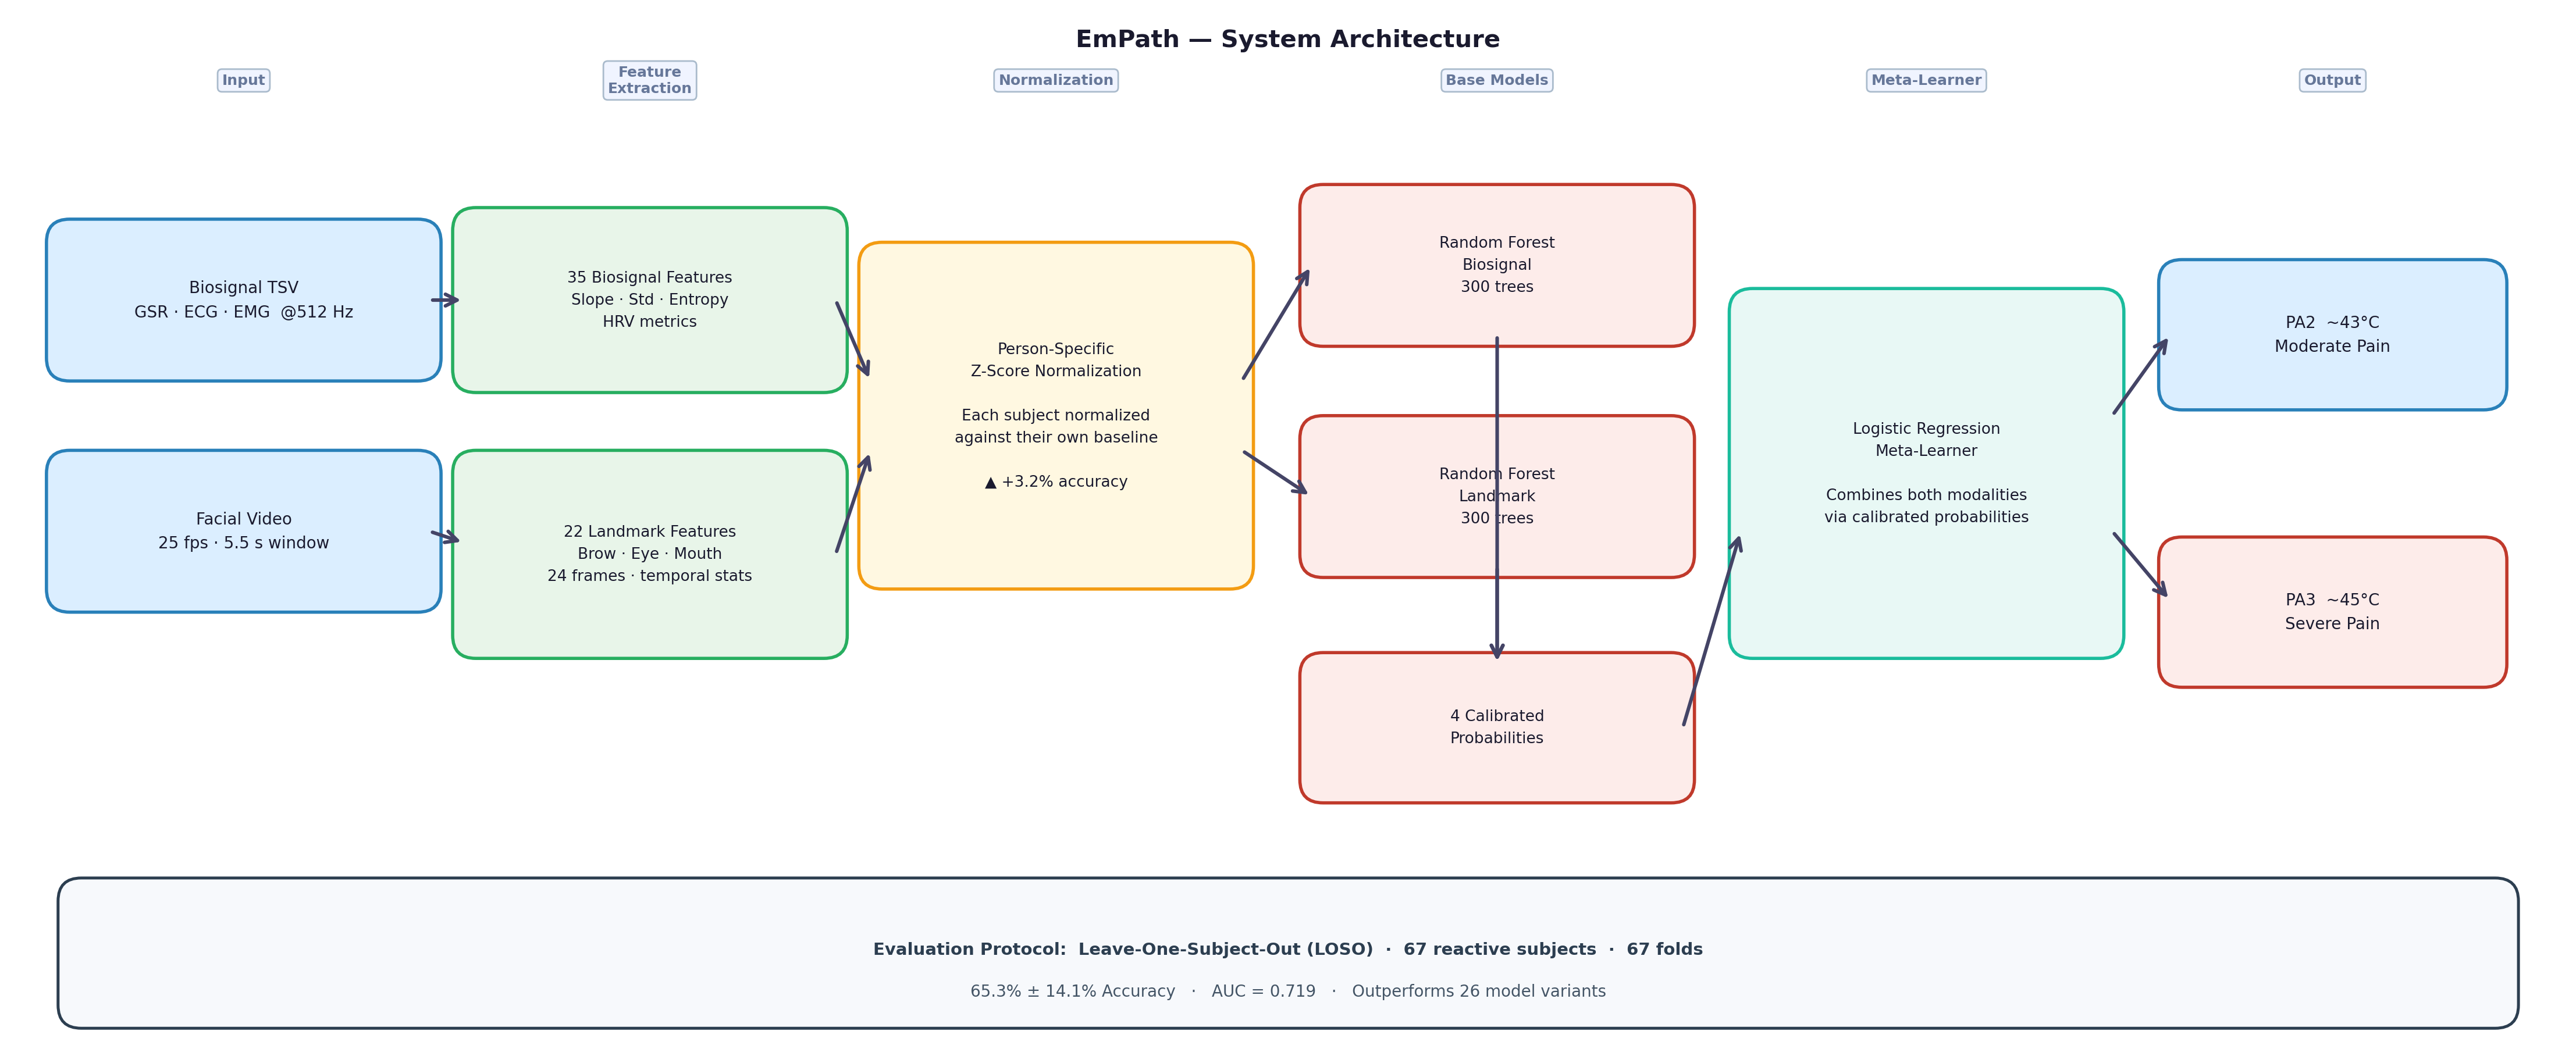
\includegraphics[width=\columnwidth]{figures/system_architecture.png}
  \caption{End-to-end data pipeline. Visual branch (left, blue): geometric
  facial landmark features. Physiological branch (right, orange): time-series
  statistics from biosignals. Both branches converge at person-specific
  $z$-score normalization before training the stacked generalization framework.}
  \label{fig:arch}
\end{figure}

\subsection{Person-Specific Normalization}

Each subject's features are transformed to zero mean and unit variance using
statistics computed \emph{exclusively} from that subject's own data. During
training folds (LOSO: all $n-1$ subjects), each subject's statistics are
computed independently before pooling the normalized training set. During test
folds (single held-out subject), statistics are computed from the subject's own
unlabeled feature values---an instance of transductive inference that does not
constitute label leakage, since statistics are purely functions of feature
values. This design choice yields a $+3.2$ percentage-point improvement over
global normalization (biosignal RF: $59.9\%$ without vs.\ $63.1\%$ with
person-norm), confirming that inter-individual physiological variability is a
primary source of classification difficulty.

\subsection{Evaluation Protocol}

All models are evaluated under LOSO cross-validation across 67 folds. In each
fold, one subject is held out for testing while the remaining 66 subjects
(2,640 samples) provide training data. No test-subject data appears in feature
normalization statistics, hyperparameter selection, or model training, ensuring
strict evaluation of cross-subject generalization. Primary metric: mean LOSO
fold accuracy ($\pm$ standard deviation across folds). Secondary metrics:
area under the ROC curve (AUC) and macro $F_1$ score.

%% ============================================================
\section{Results}
\label{sec:results}
%% ============================================================

\subsection{Overall Classification Performance}

EmPath achieves $\mathbf{65.3\%}$ mean LOSO accuracy ($SD = 14.1\%$,
$\text{AUC} = 0.719$, $F_1 = 0.653$) across 67 folds, significantly exceeding
chance ($50.0\%$; $t(66) = 10.90$, $p < .001$). Table~\ref{tab:results}
summarizes performance relative to baselines. The fusion model surpasses the
biosignal-only baseline by 2.2 pp and the landmark-only baseline by 3.9 pp,
and outperforms early (concatenation) fusion by 0.7 pp.

\begin{table}[t]
\centering
\caption{Primary performance metrics: EmPath vs.\ baselines (LOSO-67).}
\label{tab:results}
\begin{tabular}{@{}lcccc@{}}
\toprule
Model & Acc.(\%) & SD(\%) & AUC & $F_1$ \\
\midrule
Chance baseline        & 50.0 & ---  & 0.500 & 0.500 \\
Biosig. RF (no norm)   & 59.9 & 13.2 & ---   & ---   \\
Biosignal RF           & 63.1 & 11.6 & 0.668 & 0.631 \\
Landmark RF            & 61.4 & 13.1 & 0.641 & 0.614 \\
Early fusion (concat)  & 64.6 & 13.8 & 0.701 & 0.646 \\
\textbf{EmPath Stacked}& \textbf{65.3} & \textbf{14.1} & \textbf{0.719} & \textbf{0.653} \\
\bottomrule
\end{tabular}
\end{table}

\subsection{Ablation Study}

Table~\ref{tab:ablation} presents a representative selection from the 26-variant
ablation. Key patterns: (1)~random-split models dramatically overestimate
performance, confirming the importance of strict LOSO evaluation;
(2)~foundation models (BIOT, PainFormer, Tiny-BioMoE) underperform simple RF
baselines, indicating distribution mismatch between pretraining corpora and
heat-pain-elicited signals; (3)~Graph Neural Networks applied to raw landmark
coordinates (51.7\%) trail derived geometric features (61.4\%) by 9.7 pp,
confirming the value of domain-informed feature engineering over learned
graph structure at this dataset scale; (4)~Domain-Adversarial Neural
Networks~\cite{ganin2016} achieve 61.6\% alone and 64.7\% stacked, below the
non-adversarial baseline; (5)~all 26 variants converge near 65\%, strongly
suggesting an information-theoretic ceiling rather than a model-capacity
limitation.

\begin{table}[t]
\centering
\caption{Selected ablation results (LOSO-67 unless noted).}
\label{tab:ablation}
\begin{tabular}{@{}lcc@{}}
\toprule
Model Variant & Acc.(\%) & SD(\%) \\
\midrule
\multicolumn{3}{@{}l}{\textit{Single-modality baselines (random split*)}} \\
Biosignal SVM*          & 48.8 & --- \\
Biosignal MLP*          & 51.2 & --- \\
Biosignal TCN*          & 55.9 & --- \\
\multicolumn{3}{@{}l}{\textit{Foundation models (LOSO-67)}} \\
PainFormer              & 53.1 & ---  \\
BIOT                    & 54.4 & ---  \\
Tiny-BioMoE + hand feats& 61.7 & ---  \\
\multicolumn{3}{@{}l}{\textit{Single-modality (LOSO-67)}} \\
Biosignal RF            & 63.1 & 11.6 \\
Landmark RF (flat)      & 61.4 & 13.1 \\
\multicolumn{3}{@{}l}{\textit{Fusion variants (LOSO-67)}} \\
Early fusion (concat RF)       & 64.6 & 13.8 \\
Subject adaptation RF          & 65.1 & ---  \\
\textbf{EmPath Stacked Fusion} & \textbf{65.3} & \textbf{14.1} \\
\multicolumn{3}{@{}l}{\textit{Advanced architectures (LOSO-67)}} \\
GNN landmarks only      & 51.7 &  9.8 \\
DANN biosignal          & 61.6 & 10.3 \\
DANN + RF landmarks     & 64.7 & 11.8 \\
CrossMod cross-attention& 63.1 & 11.1 \\
\bottomrule
\multicolumn{3}{@{}l}{\footnotesize *Random train/test split; not LOSO.}
\end{tabular}
\end{table}

\subsection{SHAP Feature Importance}

Figures~\ref{fig:shap_bio} and~\ref{fig:shap_lm} present SHAP feature
importance rankings for both base models (TreeExplainer, full-data re-fit
on all 2,680 samples). \texttt{gsr\_slope} (mean $|\text{SHAP}| = 0.0372$) is
the dominant biosignal predictor. This is physiologically interpretable: the
sympathetic nervous system's fight-or-flight response drives a characteristic
eccrine sweat gland activation, and the slope of skin conductance rise is more
sensitive to between-condition variance than static amplitude. The top four
biosignal features are all GSR-derived, underscoring electrodermal activity as
the primary physiological discriminant for adjacent pain levels.

\begin{figure}[t]
  \centering
  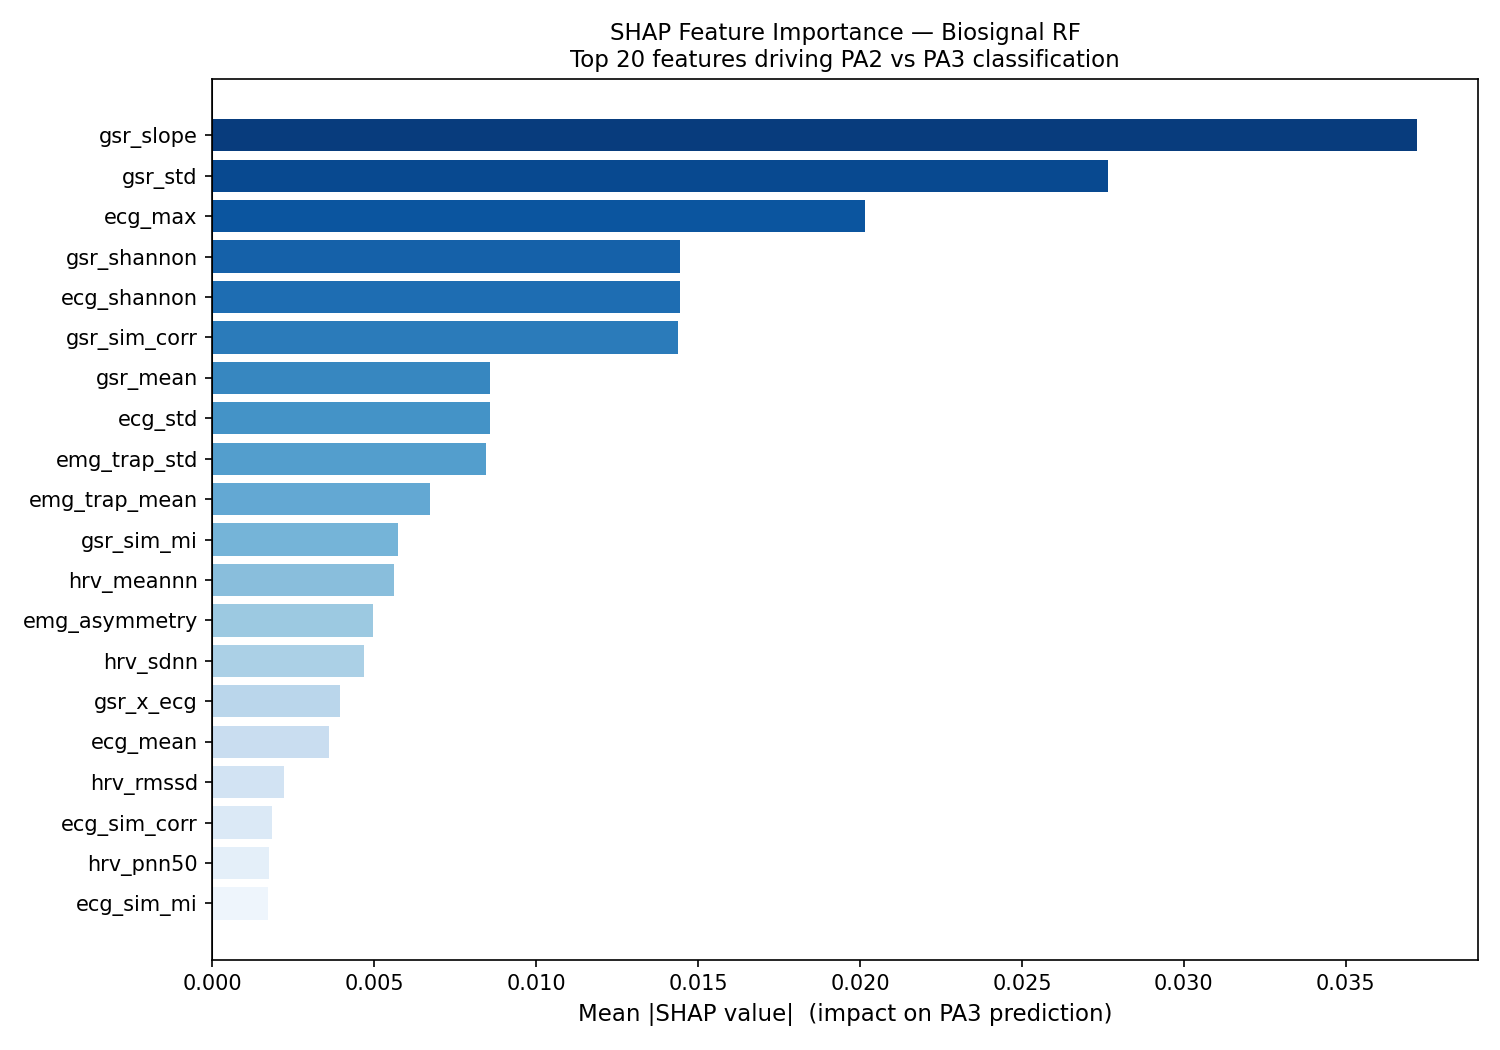
\includegraphics[width=\columnwidth]{figures/shap_biosignal_bar.png}
  \caption{SHAP feature importance for the biosignal RF base model
  (TreeExplainer, full-data fit). The top four features are all
  GSR-derived; \texttt{gsr\_slope} dominates with mean
  $|\text{SHAP}| = 0.0372$.}
  \label{fig:shap_bio}
\end{figure}

For facial landmarks, \texttt{mouth\_height\_std}
(mean $|\text{SHAP}| = 0.0289$) is dominant, encoding temporal variability of
lip separation across 24 frames---the dynamics of jaw drop and lip parting
correspond to FACS AUs~25/26~\cite{prkachin2008}. Crucially, temporal
variability features (\texttt{*\_std}) consistently outrank mean configuration
features (\texttt{*\_mean}), confirming that the dynamics of facial response,
rather than average expression state, carry the primary discriminative signal.

\begin{figure}[t]
  \centering
  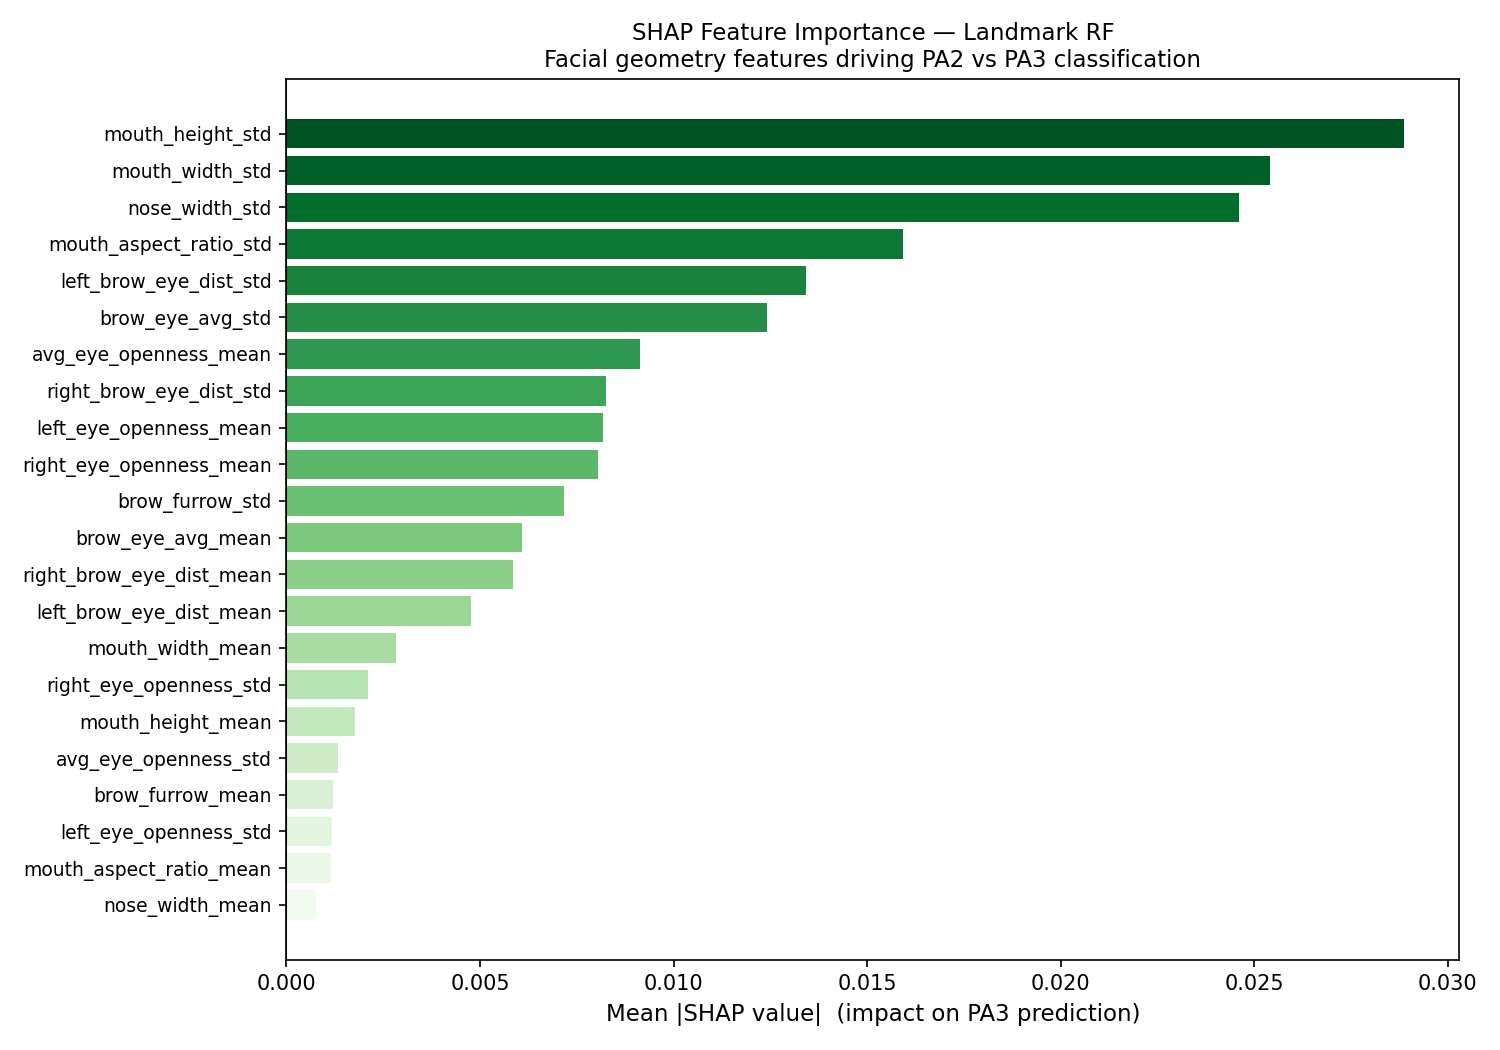
\includegraphics[width=\columnwidth]{figures/shap_landmark_bar.png}
  \caption{SHAP feature importance for the landmark RF base model.
  Temporal variability features (\texttt{*\_std}) dominate over mean
  configuration features (\texttt{*\_mean}).}
  \label{fig:shap_lm}
\end{figure}

\subsection{Per-Subject Accuracy Distribution}

Table~\ref{tab:tiers} categorizes the 67 per-fold accuracies into tiers.
Notably, 20.9\% of subjects show performance below 55\%, indicating the
model essentially fails for these individuals. At the other extreme, 9.0\%
achieve $\geq 85\%$ accuracy. This bimodal tendency is consistent with
evidence for distinct physiological responder subtypes in the affective
biosignal literature~\cite{gkikas2023}, and suggests that a personalized
system with a brief calibration phase (5--10 minutes of resting baseline
recording) could substantially improve individual-level performance.

\begin{table}[t]
\centering
\caption{Per-subject LOSO accuracy tiers ($N = 67$).}
\label{tab:tiers}
\begin{tabular}{@{}lcc@{}}
\toprule
Tier & Accuracy Range & $N$ (\%) \\
\midrule
Excellent    & $\geq 80\%$  & 14 (20.9\%) \\
Good         & 65--79\%     & 23 (34.3\%) \\
Near-chance  & 50--64\%     & 23 (34.3\%) \\
Below chance & $< 50\%$     &  7 (10.4\%) \\
\bottomrule
\end{tabular}
\end{table}

%% ============================================================
\section{Discussion}
\label{sec:discussion}
%% ============================================================

\textbf{Why stacking beats concatenation.}
The 0.7~pp advantage of stacked over early fusion confirms that preserving
modality boundaries and combining calibrated probability estimates is more
effective than mixing heterogeneous raw features. When the biosignal RF is
uncertain (probabilities near 0.5), the landmark RF occasionally provides a
more confident and correct vote, and the meta-learner learns to weight this
signal accordingly.

\textbf{Why deep learning underperforms.}
Each LOSO training fold provides only $\approx$2,640 samples, approximately 39
per training subject. Deep models with millions of parameters require orders of
magnitude more data to generalize; without it, they converge to solutions that
model individual subjects' idiosyncratic physiological patterns rather than
pain-relevant structure. This explanation is supported by the observation that
GNNs applied to raw 468-landmark coordinates (51.7\%) trail derived features
(61.4\%) by 9.7~pp---domain knowledge about which anatomical regions are
pain-relevant outperforms learned graph structure at this scale.

\textbf{Performance ceiling and its sources.}
The convergence of 26 architectural variants near 65\% strongly suggests an
information-theoretic ceiling rather than a model-capacity limitation. Three
factors constrain discriminative information: (1)~PA2 and PA3 differ by
$\approx 1^\circ$C, below many individuals' discriminable just-noticeable
difference for thermal pain~\cite{yarnitsky1995}; (2)~the 5.5-second trial
window limits reliable HRV estimation (standard guidelines recommend
$\geq 30$ seconds~\cite{taskforce1996}); and (3)~67-subject LOSO provides
insufficient diversity for subject-independent deep learning.

\textbf{Clinical implications.}
A 65.3\% accuracy represents a 15.3~pp improvement over chance, which in a
clinical monitoring context could meaningfully increase the sensitivity of
automated pain alerts for non-communicative patients. The bimodal per-subject
distribution suggests that a personalized system with a brief calibration
phase could achieve substantially higher performance for the 55.2\% of subjects
in the Good or Excellent tiers.

\textbf{Limitations.}
The BioVid database comprises 87 participants from a single German university
hospital, limiting demographic diversity. The 5.5-second window is too short
for reliable HRV estimation. Geometric landmark features discard periorbital
and forehead shape changes associated with AU6 (cheek raiser) and upper-face
pain expressions. Future work should prioritize temporal modeling of
physiological dynamics, longer recording windows, and clinical validation in
target patient populations (ICU, dementia, neonates).

%% ============================================================
\section{Conclusion}
\label{sec:conclusion}
%% ============================================================

We presented EmPath, a multimodal pain intensity detection system achieving
$65.3\% \pm 14.1\%$ LOSO accuracy ($\text{AUC} = 0.719$) on PA2/PA3
discrimination across 67 thermally reactive BioVid subjects---to our knowledge,
the first reported result under this strict evaluation protocol. Person-specific
$z$-score normalization ($+3.2$~pp) and stacked generalization
($+0.7$~pp over early fusion) are the two key design decisions. SHAP analysis
confirms physiologically grounded discriminants: \texttt{gsr\_slope} for
biosignals and \texttt{mouth\_height\_std} for facial landmarks. A 26-variant
ablation establishes the practical performance ceiling at $\approx 65\%$ for
this dataset and protocol, with deep learning and foundation models
consistently underperforming classical methods due to data sparsity under LOSO.
These findings provide a transparent, reproducible reference point against
which future adjacent-level pain discrimination methods can be benchmarked.

%% ============================================================
\section*{Data and Code Availability}
%% ============================================================

The BioVid Heat Pain Database is available upon request from the original
investigators~\cite{walter2013}. Code for feature extraction, model training,
SHAP analysis, and all 26 ablation scripts is publicly available at
\url{https://github.com/komalabelursrinivas/empath-pain-detection}.
An interactive Streamlit demonstration is accessible at
\url{https://komala-b-srinivas-empath-app-oxt9of.streamlit.app/}.

%% ============================================================
\section*{Ethical Statement}
%% ============================================================

This study uses the publicly available BioVid Heat Pain Database~\cite{walter2013},
which was collected under institutional ethics approval at the University of
T\"{u}bingen. No new human subjects data were collected for this work.

%% ============================================================
\section*{Acknowledgments}
%% ============================================================

The authors thank the Hofstra University Department of Computer Science for
computational support and access to HPC cluster resources (SLURM).

%% ============================================================
%% BIBLIOGRAPHY
%% ============================================================
\bibliographystyle{ACM-Reference-Format}
\bibliography{empath}

\end{document}
